\section{Solution}
We have discussed some information about the problem of cyberbullying, and have have concluded that a lack of reporting appears to exacerbate the problem. The bully gets encouraged because of he or she is not reported to the authorities, and hence bullying never stops. If the victim or any of the witnesses start reporting to a reliable source that can either block the bully from posting comments about others or can actually catch the bully, then the problem of cyberbullying can be controlled to a far extent.

\subsection{Centralized Reporting Platform}
Our aim is to provide a reliable reporting platform to the victims or witnesses where they can report the incidents of cyberbullying. This platform is a web portal which could directly be under the control of an authoritative department such as police or any concerned government official. This initiative would require the authorities to work in close contact with the administrative teams of various websites. With the collaboration of admin team and the police department, all the reported incidents can be tracked down and hence the bullies can be accordingly punished. This would instill confidence in people that they have someone to look forward to in case they witness or experience any kind of cyberbullying.

\subsubsection{User Side of CBRP}
Let us have a look at the Cyber Bullying Reporting Platform (CBRP). Figure \ref{Figure_1} is a sample image of the web portal. 


\begin{figure}[h]
\centering
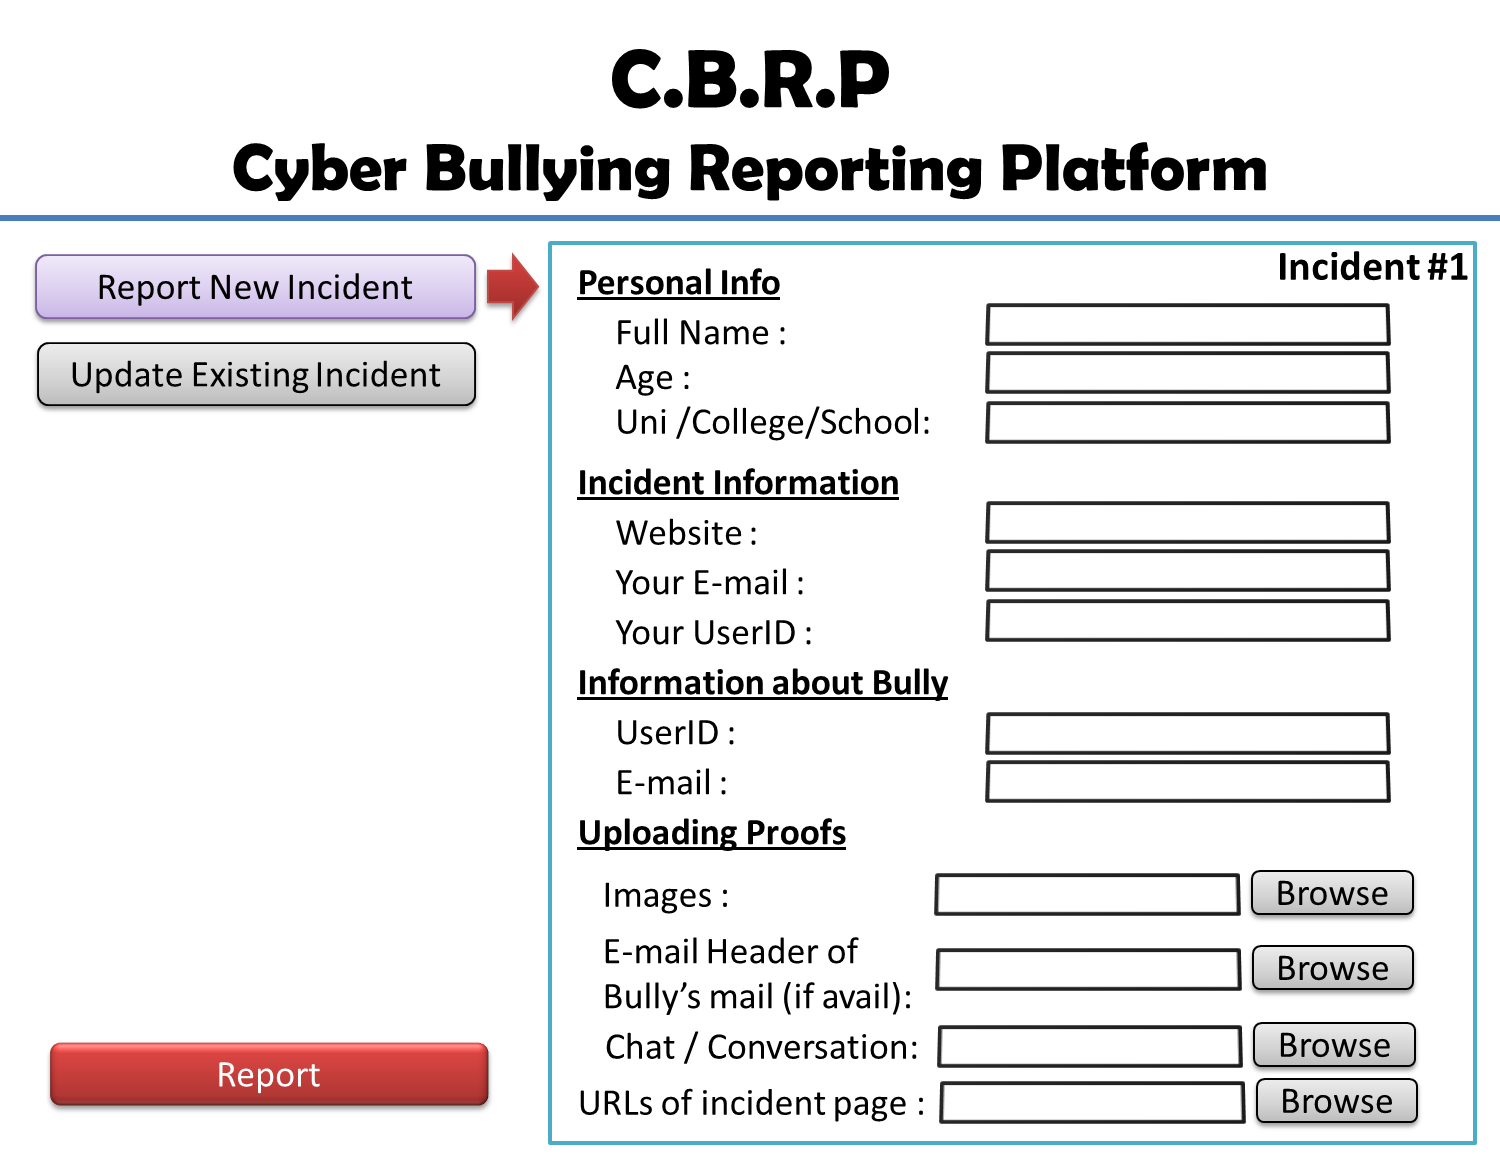
\includegraphics[width=0.8\textwidth]{images/Figure_1}
\caption{}
\label{Figure_1}
\end{figure}


CBRP is a basic web portal where the victims or the witnesses can report the incident. They will be required to create a basic username on the website which would keep track of all the incidents related to that user. The form contains personal information like name, age and current university/college/school that the person is attending. The basic purpose of getting this information is to narrow down the scope of possibilities to find the bully. All the information provided will be used to track down the bully.
 
Further the portal asks for information about the source of the incident like the website on which the unwanted content is published. The victim’s email Id and username is required and also that userID (or preferably the email address) from which the messages are being sent. All this information would be made visible to the admin of the corresponding website to track down the provided ids and verify if the bullying is being undertaken.
 
In addition to these there is a provision of uploading exact proofs in the form of images or messages being sent by the bully. All the images posted or the text messages delivered can be uploaded by the reporter and later used by the authorities to verify the bullying incident and use as a proof against the bully. Even the email headers (if possible) can be also uploaded by the informer as the headers contain a lot of information about the mail sender. It also has information about the IP address of the person sending the message. With an email header it becomes far easy to get hands on the bully.

This form can be filled by the victims themselves or by any witness of cyber bullying. All the incidents will be under one thread with the created username. The Personal information will not be shared with the admin of websites. Only the information required for tracking and verifying will be shared. All the information will be reported to the higher authority in charge, may be police department. So that in case the bully continues and the seriousness is grave, police can use all the necessary information uploaded to track and catch the bully.

\subsubsection{Acknowledgement Screen}
After the incident is reported the user is presented with an acknowledgement screen. The snapshot of this screen is shown in Figure \ref{Figure_2}.


\begin{figure}[h]
\centering
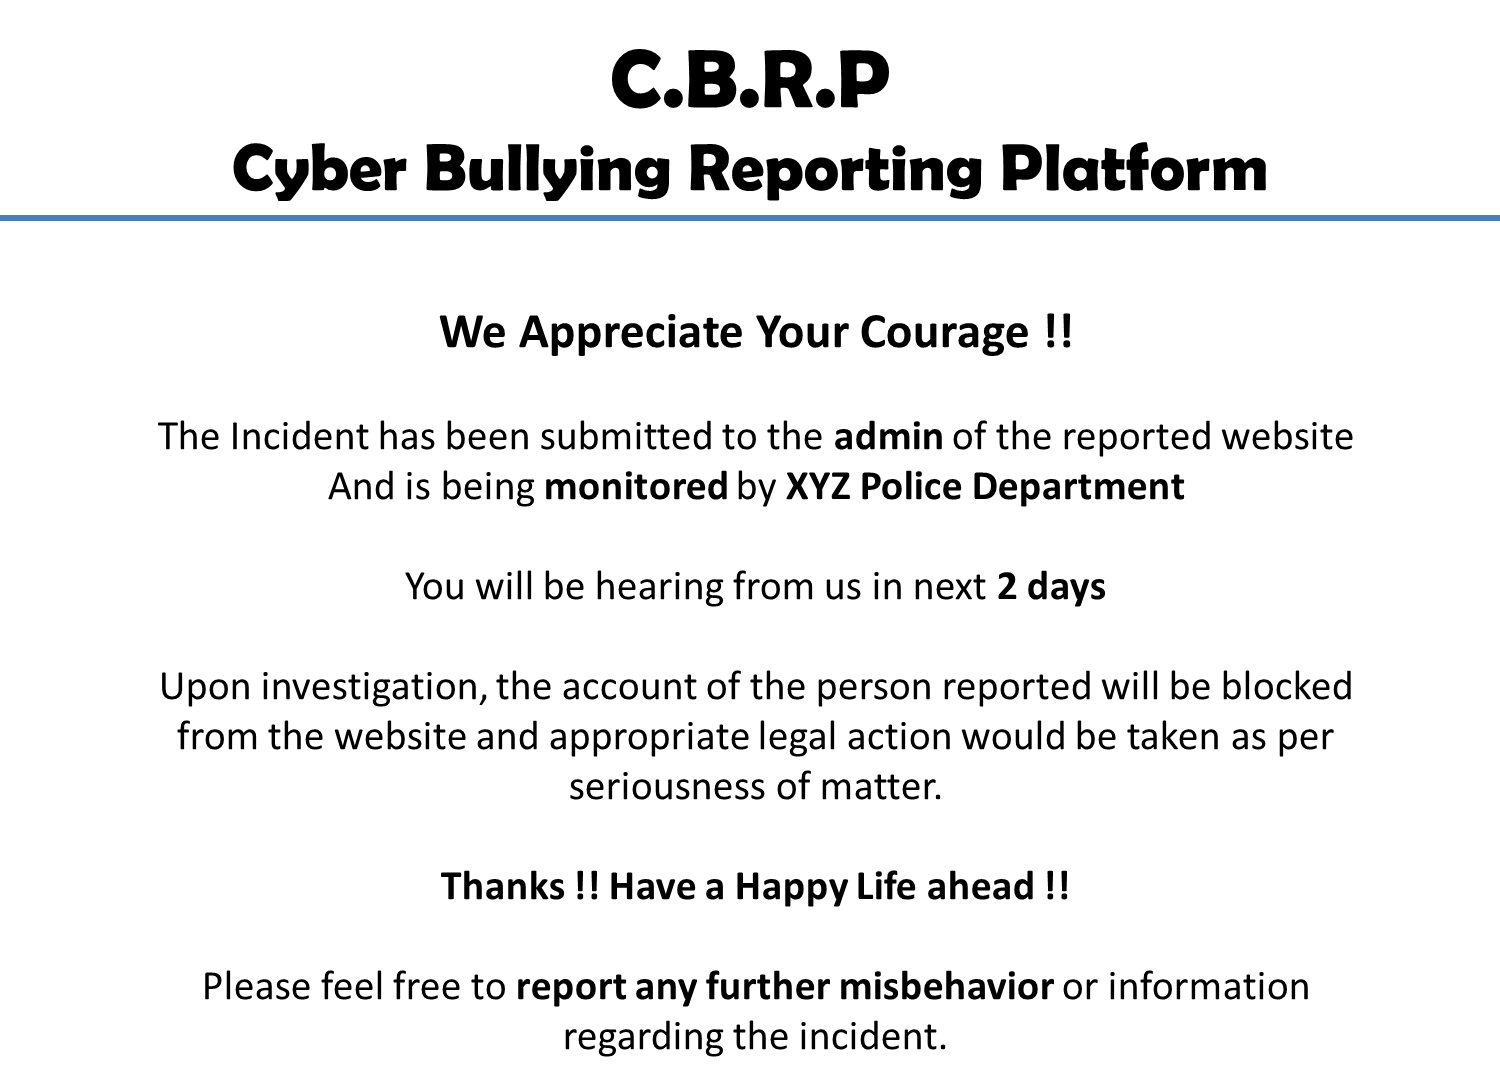
\includegraphics[width=0.8\textwidth]{images/Figure_2}
\caption{}
\label{Figure_2}
\end{figure}



This screen solves various purposes like:
\begin{enumerate}

\item
It provides \textbf{encouragement} to the person who has reported the incident. The immense courage of the person is appreciated. 
\item
It provides \textbf{satisfaction} to the person when he/she knows that administrators and the concerned police department will be looking into the case.
\item
Thirdly, it \textbf{provides} a hope that the case will be taken care in specified number of days. So this provides a big hope to the person who is being harassed.
\item
This page, further \textbf{motivates} the person for providing any other information which could be helpful in catching the bully ASAP.
\end{enumerate}

\subsubsection{View for Authoritative Department}
So far, we have seen the user’s side of the web page. Let us now have a look at the portal available to the police department or other authority in charge. The snapshot is shown in Figure \ref{Figure_3}.


\begin{figure}[h]
\centering
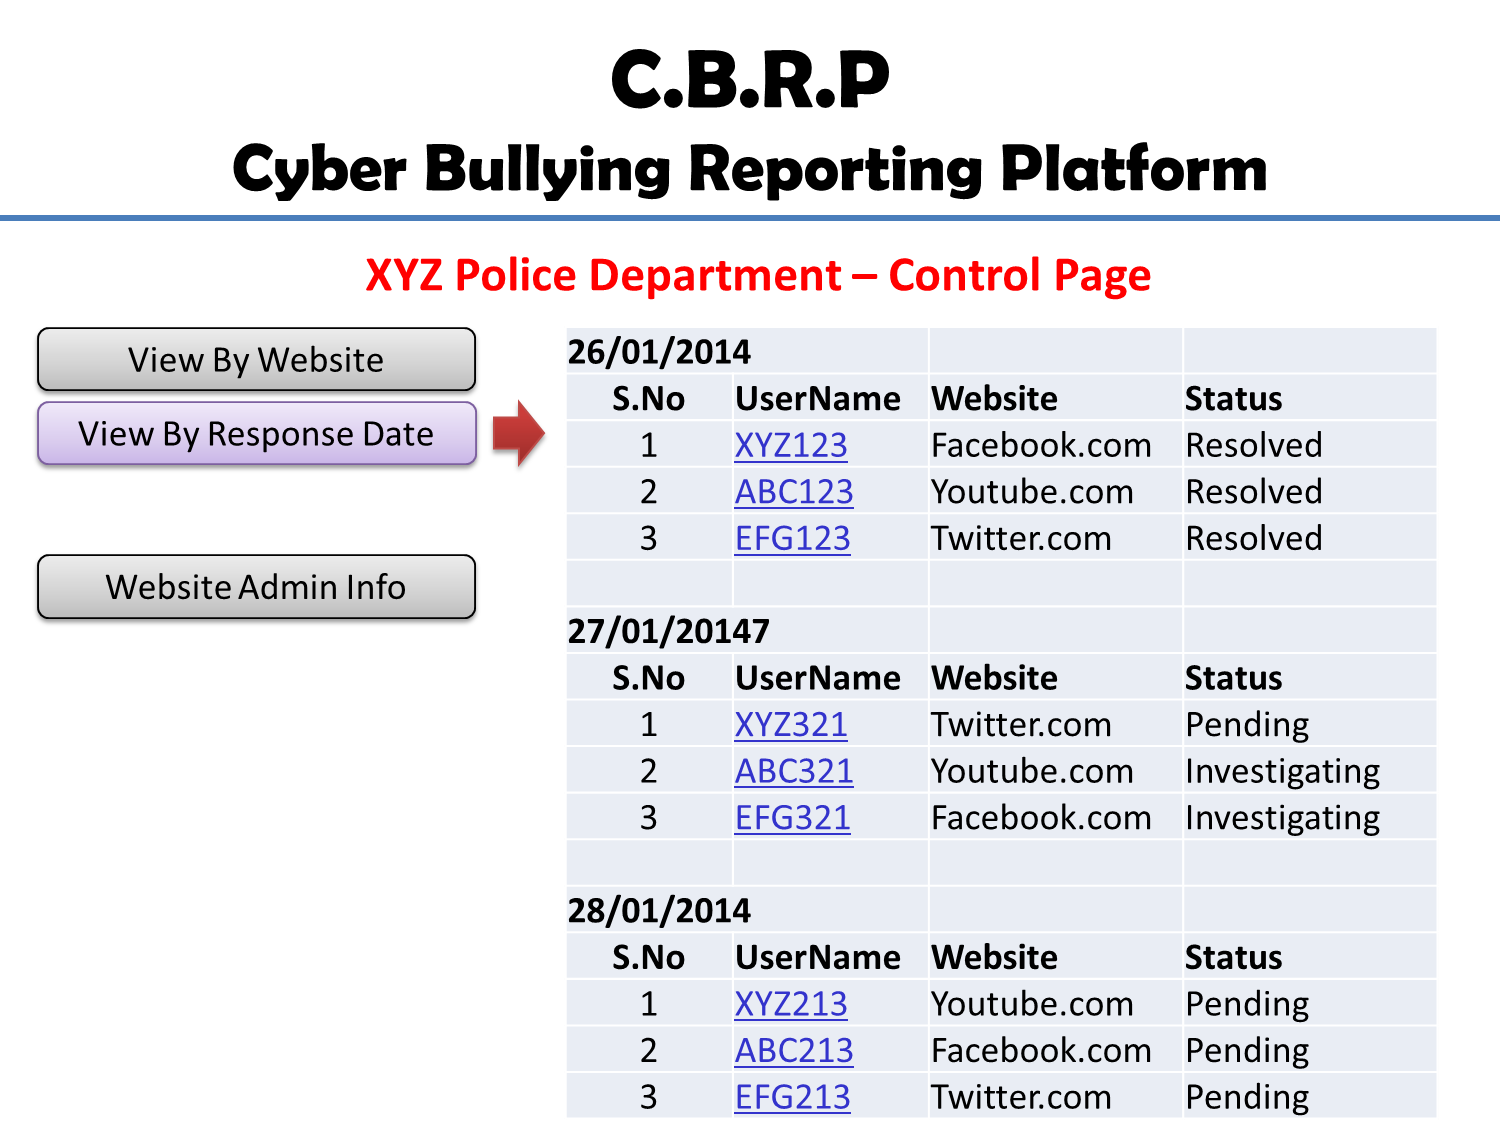
\includegraphics[width=0.8\textwidth]{images/Figure_3}
\caption{}
\label{Figure_3}
\end{figure}



The police department or any other authority in charge would have access to this page. They can get the list of incidents arranged by website names or by response date. Since this is trusted authority so they can have access to full information provided by the victim. The whole profile information along with all the materials uploaded under the same thread would be available to the department. In order to have a close monitoring on the response dates, they can directly contact the admin teams of the corresponding websites. This check would make the things moving at the end of website’s admin team and will surely help to take action on time.  It also provides all the proofs to the police so they can track the person in case further bullying continues from the same person. This could help in producing proofs in legal proceedings as well.

\subsubsection{View for Website Admin Team}
Similar to the police department section, there is an admin side of the portal as well. This would be available to the admin of the website to trace the incidents. A glimpse of the page is shown in Figure \ref{Figure_4}. 

\begin{figure}[h]
\centering
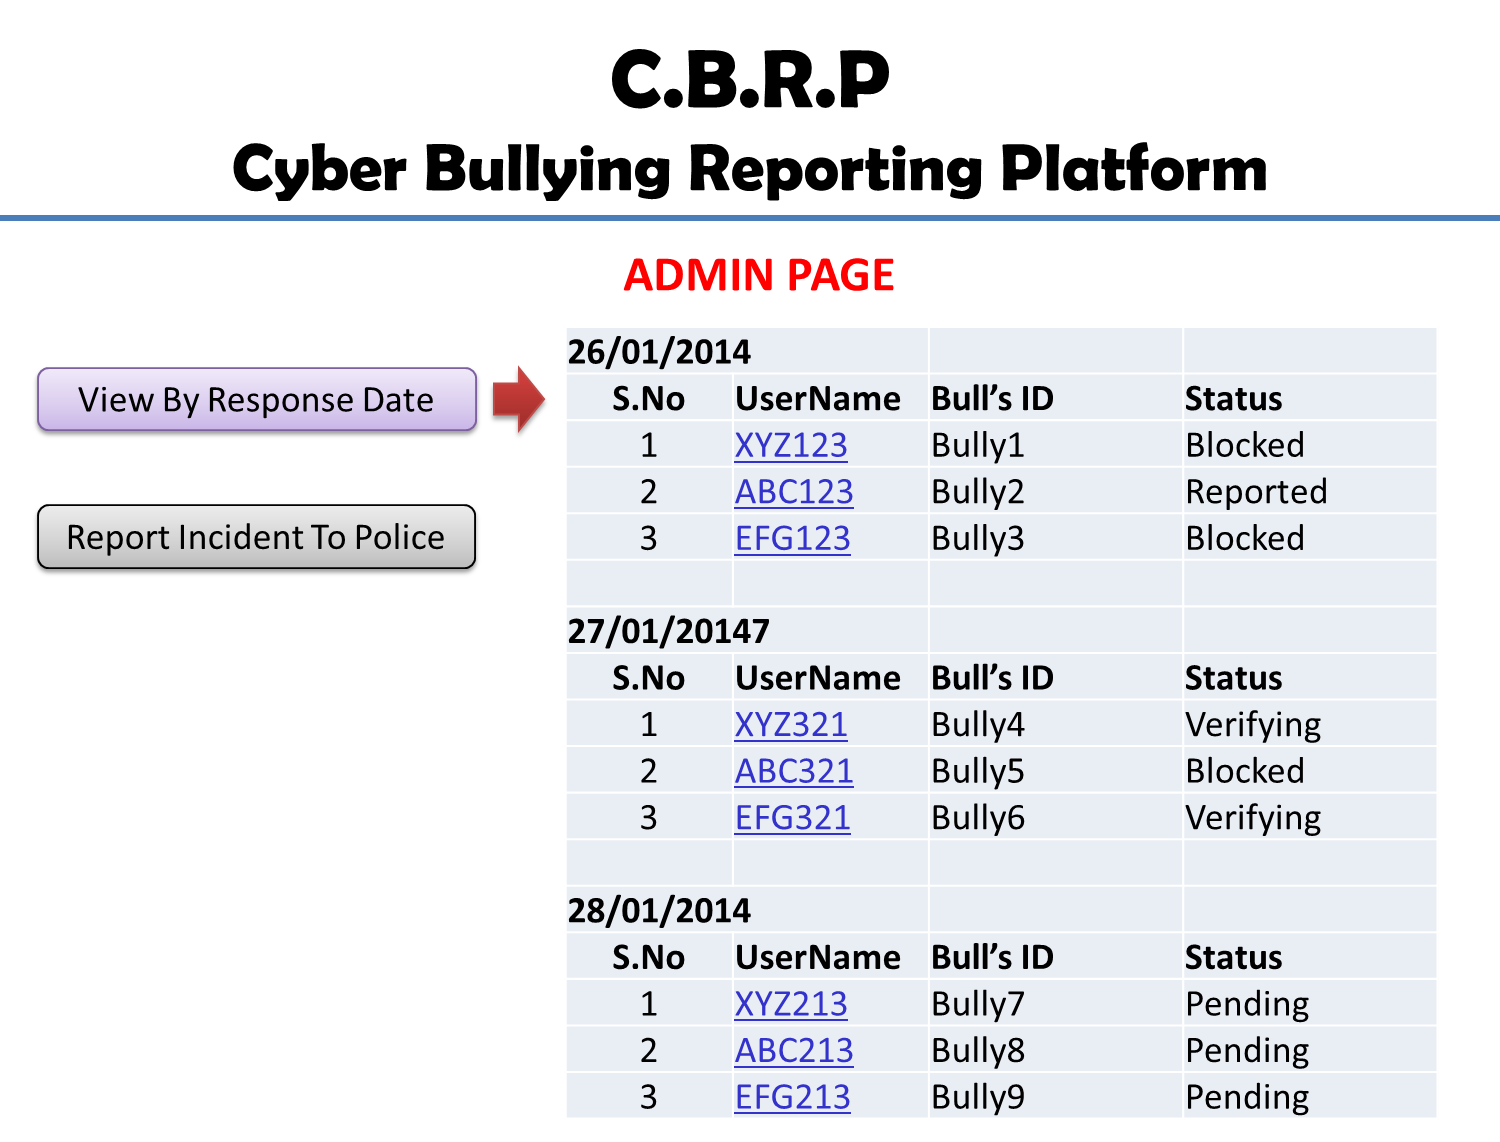
\includegraphics[width=0.8\textwidth]{images/Figure_4}
\caption{}
\label{Figure_4}
\end{figure}

The working of this whole concept drills down to the responsibility of the web admin of the website. All the necessary information uploaded by the victim is available to the admin. Although the personal information can be hidden from the admin, upon request, but rest all the information necessary for tracking is available for use. The admin is responsible for first of all verifying the information uploaded by the victim. He has to make sure that the information provided is actually present on the website so that the incident reported is not a fake. Then he can track down the id provided and can back track the IP of the person. As a second step, he needs to block any further communication on the website from the same IP. This way further harassment to the victim is stopped. Also a feedback can be sent to the victim at this point that the bully will not be able to harass the victim from the reported user ID and from any other id used on same IP address. 

As a next step he can inform the police department about the IP or the person’s identity and thereon police can handle the case. In case the bully is using different websites for harassing, still he can be tracked because of this centralized platform. Since police has great authority, they can ask the ISPs to block the Internet access of the person so that bully might not be able to use the network further. This would cut down the bully from doing this crime further. 

\subsection{Impact}
CBRP, if used actively can minimize and can put a stop to the cyberbullying as soon as it starts up on the web. Larger teams of professionals can be used to monitor the website and track down the bullies in no time. It will also be really easy to put them under criminal trial with all the proofs collected against them. The more the incidents this site would be able to stop, the more trust will be built up in the people and lesser the incidents of cyberbullying will be.

Hence, together with the courage of the people to report the incidents and the active participation of police and the admin teams of websites, the cases of cyberbullying can be drastically reduced and the bully can be given their deserved punishment.
